\chapter{Conversion of seismic fragility and vulnerability models to alternative intensity measures for regional risk analysis}

This chapter is based on the following publication:
\begin{quote}
    \bibentry{OReilly2026-ffconversion}
\end{quote}


\section{Introduction}
Seismic risk analysis involves using fragility and loss models to probabilistically describe the potential negative outcomes resulting from earthquake events. These include damage evaluations like structural collapse during seismic shaking, where fragility functions are required, or losses via vulnerability functions. More formally, fragility functions describe the probability of a structure exceeding a given \ac{DS} at a certain intensity of shaking, $P[DS>ds\mid IM=im]$. Likewise, a vulnerability function describes the expected value of loss for a given level of shaking, $E[L\mid IM=im]$. This definition of loss typically refers to economic loss but can be extended to other consequences such as indirect losses, casualties or business interruption. The conditioning value of intensity in these fragility (or vulnerability) functions is characterised by an \ac{IM}, which can have various types, including classical definitions like \ac{PGA} or spectral acceleration at a given period, $Sa(T)$, or even more generalised definitions like macroseismic intensity. The choice of this \ac{IM} depends on factors such as structure typology, application purpose, and data availability. The suitability of \acp{IM} can be evaluated using several criteria, typically described as sufficiency, efficiency, practicality, and lack of bias. The result of this wide range of \ac{IM} choices, and the means with which to evaluate their suitability, often yields libraries of fragility (or vulnerability) functions from typology-specific studies, in many cases possessing slightly different \ac{IM} definitions. 

When performing regional risk analysis, where large portfolios of assets are geographically spread across different locations, \acp{GMF} are simulated based on a stochastic event set. These are combined with catalogues of functions that represent the portfolio, herein referred to as models, to estimate the negative consequences such as loss. Doing this with fragility (or vulnerability) models defined using a plethora of \acp{IM} can become challenging. If the assets can be considered independent, their losses are assessed independently using individual \ac{IM}-specific \acp{GMF} and the total loss for the entire portfolio is found by summing all the individual contributions. However, in situations where assets cannot be considered independent, difficulties arise since it means that several cross-correlated \acp{GMF} must be simultaneously generated to evaluate the assets collectively. It is not only computationally very demanding to handle a large spatial covariance matrix, but the required models to generate these cross-correlated \acp{GMF} are seldom available \citep[e.g.,][]{MonteiroOReilly2026}. However, it should be noted that procedures based on conditional hazard that simplify the modelling of \acp{GMF} do exist \citep[e.g.,][]{Weatherill2015}, although these come with the penalty of approximating some correlations \citep[e.g.,][]{Goda2008}. Examples of where such consideration would be needed are for critical infrastructures such as power, gas, water and bridge networks with cascading effects \citep[e.g.,][]{Franchin2015, Esposito2015, Abarca2022a, Abarca2023}, or when the structure-to-structure damage correlation between buildings is considered \citep[][]{Heresi2022, Mejia2025}. 

Alternatively, it is often simpler and more computationally efficient to define fragility (or vulnerability) models in terms of common \acp{IM} so that a single \ac{GMF} can be used in consequence estimation. This would have the added benefit that fragility/vulnerability models from different sources can be directly compared to visually assess their differences and suitability for specific taxonomies. Standard definitions are typically used, such as \ac{PGA} or spectral acceleration at a specific period like $Sa(T=0.5s)$. For example, \citet{Rosti2021} used \ac{PGA} to define fragility models, opting for a practical and pragmatic approach, despite the known issues of sufficiency, efficiency and bias that have been widely reported in the literature \citep[e.g.,][]{ShomeEtAl1998, MehdizadehEtAl2017, GhimireEtAl2021, OReilly2021}. Also, the \ac{GEM} global \citep{Martins2021-BEE} and the \ac{ESRM20} \citep{ESRM20} models use several definitions of $Sa(T)$ in their risk models that somewhat mediate these issues that persist with \ac{PGA}. Nonetheless, these generalised definitions of \ac{IM} for fragility/vulnerability models still contrast structure-specific \acp{IM} like spectral acceleration at the predominant period of vibration $Sa(T=T_1)$ or other ad hoc definitions, which often boast increased accuracy through their detailed scrutiny. Furthermore, advancements in vulnerability modelling have indicated that there are several so-called next-generation \acp{IM} such as average spectral acceleration, $Sa_{avg}(T)$ \citep[e.g.,][]{Eads2015, Kazantzi2015}, or filtered incremental velocity, $FIV3(T)$ \citep{Davalos2019}, that have demonstrated much improved accuracy and explanatory power with respect to classic \acp{IM} like \ac{PGA} or $Sa(T)$. Despite these advancements in vulnerability modelling, their use on a regional scale remains limited to date.

Unless systematic vulnerability model development for a wide range of taxonomies is collectively carried out, such as \citet{Martins2021-BEE} and \citet{ESRM20}, risk modellers often face the issue of how to rationally use several different \ac{IM} definitions in their fragility/vulnerability models when looking to comparatively assess them, or collectively apply them to inter-dependent structural networks. Furthermore, using such generalised and regional approaches to vulnerability modelling, they cannot benefit from the dozens of individual models that are developed for individual research groups based on detailed analysis for specific typologies and \ac{IM} definitions. Faced with this, the analyst's choices are then to follow three different strategies, assuming the analyst cannot segregate the analysis and perform independent evaluations. The first is to use a single \ac{IM} for all fragility (or vulnerability) functions, and estimate consequences from a single \ac{GMF} with these. The second involves using several and more optimised \acp{IM} for every fragility/vulnerability function, and estimating consequences from several cross-correlated \acp{GMF} with these. This is despite these cross-correlated models being seldom available and difficult to generate \citep{MonteiroOReilly2026}, although \citet{Monteiro2026b} have recently proposed a spatial correlation model that greatly reduces this challenge in practical implementation. Lastly, the third approach is to adopt fragility (or vulnerability) functions from several ad hoc sources, each potentially using a different \ac{IM}, and convert them to a single generalised \ac{IM}. This would significantly increase the computational efficiency of regional analysis since it would require only a single \ac{GMF} type to be simulated. Furthermore, the generalised \ac{IM} could potentially take forms other than the classic \ac{PGA} which has persisted for several decades.

This paper discusses this last issue in detail, examining past research on model conversion and exploring the topic further to form practical advice for risk modellers. Some methods for conversion of fragility functions have been previously proposed, but have focused on the conversions between traditional intensity measure definitions (e.g., $Sa(T)$ and \ac{PGA}) via different simplified schemes. One of the most notable contributions was provided by \cite{Suzuki2020}, who employed a total probability approach. However, to date no study has thoroughly investigated conversions beyond these spectral-based \acp{IM} and next-generation \acp{IM} that have emerged as promising alternatives in recent years. The present study builds upon these foundational insights, but differs in scope and objectives. While \cite{Suzuki2020} primarily focused on the formulation of fragility conversion using scalar and vector-valued intensity measures, as well as on the accuracy of such conversions under controlled settings, this work adopts a risk-modelling perspective aimed at providing practical guidance for risk modellers. In doing so, it explores a range of conversion settings and methods based on a single \ac{IM}, reflecting the fact that the vast majority of fragility functions available in practice are developed using a single \ac{IM}. In addition, other more simple approaches based on assumptions of uniform hazard and uniform risk equivalence are trialled to investigate whether any practical usage can be made of these for \ac{IM} conversion strategies in practical application. In particular, this paper (i) systematically compares multiple conversion strategies in terms of both accuracy and practical effort with 2,260 individual cases, (ii) examines the influence of hazard disaggregation detail and \ac{IM} efficiency on conversion reliability, (iii) extends the analysis to next-generation \acp{IM}, and (iv) explores the direct conversion of vulnerability models in addition to underlying fragility functions. Through applications to 2,260 individual cases that give a more holistic view of the problem being tackled, the paper provides practical guidance for risk modellers on when and how \ac{IM} conversion can be reliably applied, and where its limitations should be acknowledged.


\section{Review of existing conversion methods}\label{sec:review}

\subsection{Uniform hazard equivalence}\label{sec:uniform-hazard-equiv}
The need to compare and cross-evaluate different fragility contributions has been known for several years. This was highlighted in the SYNER-G project \citep{Pitilakis2014} in Europe when \citet{Silva2014} proposed a fragility function manager tool to collect and compare fragility functions developed using different methodologies from various sources in the literature. While the objective was to create a centralised database and resource for risk modellers, it also addressed the issue regarding the lack of \ac{IM} uniformity across the available fragility functions. \citet{Silva2014} proposed a scaling factor based on the 2006 \ac{IBC} design spectrum \citep{IBC2006} that is applied to the fragility function's median value, and illustrated in Figure \ref{fig:uniform-hazard-conversion}, although no detailed studies were conducted to verify the accuracy of such approach. Similar strategies were proposed for \ac{PGV} and spectral displacement. \citet{OReilly2020} also proposed a similar methodology that was instead based on a comparison of the \ac{IM} hazard curves resulting from \ac{PSHA}, also shown in Figure \ref{fig:uniform-hazard-conversion}. The main advantage of this over the \citet{Silva2014} approach is that a more refined definition of the \ac{IM} hazard is employed and non-$Sa(T)$-based \acp{IM} can also be considered. Although it involves slightly more complex input data, the same underlying approximation remains, and no rigorous testing was carried out by the authors to verify the accuracy of such approach, at least with respect to simpler version proposed in \citet{Silva2014}.

\begin{figure}[htbp]
    \centering
    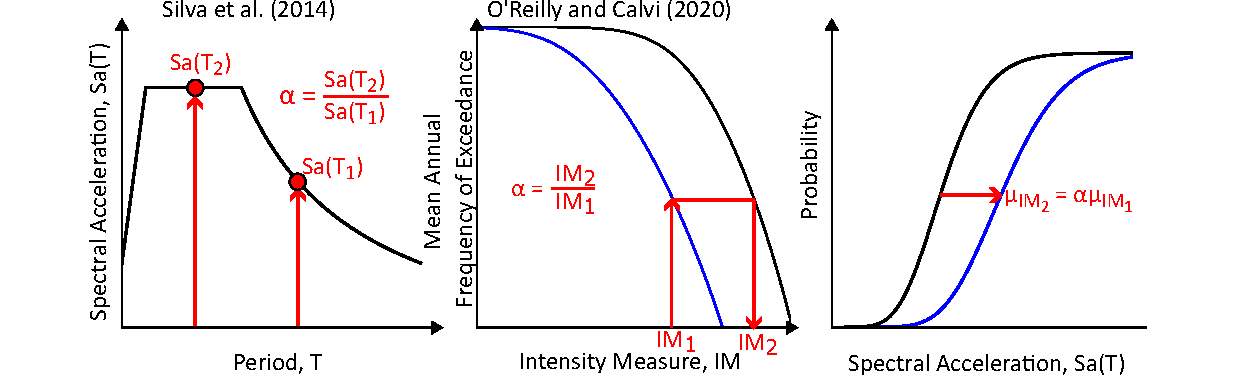
\includegraphics[width=0.9\textwidth]{figs/uniform-hazard-conversion.pdf}
    \caption{Illustration of the uniform hazard conversion methodologies described in \citet{Silva2014} and \citet{OReilly2020}}
    \label{fig:uniform-hazard-conversion}
\end{figure}

These approximate approaches are based on equivalent uniform hazard and the assumption of equal variability among the two fragility functions (i.e., the original and the converted fragility function). This means that if an analyst has a fragility function defined in terms of $Sa(1s)$ via a lognormal distribution with median $\eta$ and dispersion $\beta$, and wishes to convert it to $Sa(0.5s)$, they would simple keep the same dispersion $\beta$ and linearly scale the median value by the factor $\alpha$ (Figure \ref{fig:uniform-hazard-conversion}). The median intensity is therefore scaled based on its relative \ac{UHS}-based value. It neglects aspects of differences in variability for the \acp{IM} themselves, along with potentially different rupture contributions, and assumes all \acp{IM} are equally efficient, which is known not to be the case.

\subsection{Uniform risk approach}\label{sec:uniform-risk-equiv}
Building on the uniform hazard approach, a risk-consistent approach is trialled in this study. It is based on the fact that risk, or more formally the \ac{MAFE}, $\lambda$, of a \ac{DS} is unique for a given structure and site location regardless of the conditioning \ac{IM} employed. This was initially shown by both \citet{Bradley2012a} and \citet{Lin2013_pt1} and requires that the \ac{IM} employed is efficient, sufficient and unbiased, and that the ground motion records used in the analysis are hazard-consistent. 

If the fragility function is represented via a lognormal distribution with median and dispersion, $\eta$ and $\beta$, and the hazard curve is represented as a log-linear relationship $H=k_0im^{-k_1}$, \citet{Cornell2002} solved for $\lambda$ as shown below: 
\begin{align}
    \label{eq:cornell2002}
    \lambda_{DS} &= \int_0^{+\infty} P[DS\mid IM=im]\mid dH(IM)\mid \\
    &=k_0\eta^{-k_1}\exp\left(0.5k_1^2\beta^2\right)
\end{align}
\noindent and since $\lambda_{DS}^{IM_1}$ can be taken as equal to $\lambda_{DS}^{IM_2}$ for two different \acp{IM}, this equivalence is extended here to give:
\begin{equation}
    \lambda_{DS}^{IM_1} = \lambda_{DS}^{IM_2}
\end{equation}
\begin{equation}
    k_{0,IM_1}\eta_{IM_1}^{-k_{1,IM_1}}\exp\left(0.5k_{1,IM_1}^2\beta_{IM_1}^2\right) =k_{0,IM_2}\eta_{IM_2}^{-k_{1,IM_2}}\exp\left(0.5k_{1,IM_2}^2\beta_{IM_2}^2\right)
\end{equation}
\begin{equation}
\label{mafe-uniform-risk}
    \eta_{IM_2} = \left(\dfrac{k_{0,IM_1}\eta_{IM_1}^{-k_{1,IM_1}}\exp\left(0.5k_{1,IM_1}^2\beta_{IM_1}^2\right)}{k_{0,IM_2}\exp\left(0.5k_{1,IM_2}^2\beta_{IM_2}^2\right)}\right)^{\frac{-1}{k_{1,IM_2}}}
\end{equation}
  
Typically, the parameters of one fragility function, $\eta_{IM_1}$ and $\beta_{IM_1}$, are known, meaning that a single equation is solved for two parameters, $\eta_{IM_2}$ and $\beta_{IM_2}$. A simple approach may be to assume a fixed value of dispersion $\beta_{IM_2}$ and solve for $\eta_{IM_2}$, which will be trialled here. In addition, the second-order development of \citet{Cornell2002}'s solution in Equation \eqref{eq:cornell2002} proposed by \citet{Vamvatsikos2013} can also be utilised for improved accuracy, and will be utilised here. 

\subsection{Proxy structure analysis}
\citet{KaraferisVamvatsikos2022} presented a novel method to convert fragility functions via proxy structure analysis. This requires developing a equivalent \ac{SDOF} structure and the assumption of fundamental properties like period, strength and \ac{DS} definition. Analysts must perform many trials and iterate towards identifying an equivalent \ac{SDOF} structure that would result in the same fragility function as the candidate fragility to be converted. Once identified, this equivalent \ac{SDOF} structure's analysis results can be recomputed in terms of the target fragility function \ac{IM}. This is essentially doing a conversion of a proxy structure that is intended to represent the actual original fragility function and does not actually work on the original fragility function directly. It also requires little to no hazard information to implement, beyond selecting suitable ground motions for the \ac{SDOF} analysis making it an attractive alternative. \citet{KaraferisVamvatsikos2022} conducted several case studies and noted a good overall performance of the methodology. 


\subsection{Total probability approach}\label{sec:total-probabaility}
The previous methods each rely on simplifying assumptions regarding hazard, risk and uncertainty to devise an equivalence between \acp{IM}. To address this, proposals were made based on an application of the total probability theorem as follows:
\begin{equation}
    \label{eq:total_probability_basic}
    P[DS \mid IM_2] = \int_{IM_1} P[DS \mid IM_1] f_{IM_1 \mid IM_2} \, \mathrm{d}IM_1
\end{equation}
where $P[DS \mid IM_1]$ is the original fragility function based on $IM_1$, and $f_{IM_1 \mid  IM_2}$ is the conditional distribution of $IM_1$ given $IM_2$ to result in the converted fragility function $P[DS \mid IM_2]$. This was initially presented in \citet{Michel2018}, albeit with an error\footnote{\citet{Michel2018} mistakenly wrote the conditional distribution term in Equation \eqref{eq:total_probability_basic} as $f_{IM_2 \mid IM_1}$ instead of $f_{IM_1 \mid IM_2 }$} which was later noted and corrected by \citet{Suzuki2020}, who then further expanded and tested this formulation with 24 conversion cases of $Sa(T)$, which \citet{Michel2018} did not conduct. 

It is well-known from ground motion selection studies that the conditional distribution $f_{IM_1 \mid IM_2}$ depends on the underlying rupture parameters. Therefore, \citet{Suzuki2020} further extended Equation \eqref{eq:total_probability_basic} to include the magnitude, $M$, and rupture distance, $R$, as follows:
\begin{equation}
    \label{eq:suzuki_extension}
    P[DS \mid IM_2] = \int_{IM_1}\int_{M}\int_{R} P[DS \mid IM_1, M, R] f_{IM_1, M, R \mid IM_2} \, \mathrm{d}IM_1 \, \mathrm{d}M \, \mathrm{d}R
\end{equation}
where the conditional distribution term $f_{IM_1, M, R \mid  IM_2 }$ was rearranged to a more familiar format of:
\begin{equation}
    \label{eq:suzuki_eq2b}
    f_{IM_1, M, R \mid IM_2} = f_{IM_1 \mid IM_2, M, R}f_{M, R \mid IM_2}
\end{equation}
where $f_{IM_1\mid IM_2, M, R}$ is the conditional distribution of $IM_1$ given $IM_2$ and the rupture parameters $M$ and $R$. This conditional distribution is already widely used in the \ac{CS} or \ac{GCIM} ground motion selection approaches \citep{Lin2013_pt1, Bradley2010a}. The $P[DS \mid IM_1, M, R]$ term implies that the fragility function is also a function of rupture parameters $M$ and $R$. For most \acp{IM}, these are assumed to be sufficient \citep{Luco2007a} and hence independent of rupture parameters, meaning it can be simply written as $P[DS \mid IM_1] $ herein. The $f_{M, R \mid IM_2}$ term is computed via the disaggregation of the \ac{PSHA} results for $IM_2$ in terms of $M$ and $R$. \citet{Suzuki2020} noted that this strictly refers to the \textit{occurrence} of $IM_2 = im_2$ and not its \textit{exceedance} $IM_2 > im_2$ as is typically done. Interested readers are referred to \citet{Fox2016} for further information on the implications of either approach. While magnitude and distance are pertinent parameters from the hazard disaggregation that impact the conditional distribution $f_{IM_1, M, R \mid IM_2}$, a further step to generalise and include all scenario parameters (e.g., soil condition, rake, hypo-central depth) and \acp{GMM} is proposed here and are collectively termed $Rup$ through the generalised form:
\begin{equation}
    \label{eq:proposed-ff}
    \begin{aligned}
        P[DS \mid IM_2] &= \int_{IM_1}\int_{Rup} P[DS \mid IM_1] f_{IM_1, Rup \mid IM_2} \, \mathrm{d}IM_1 \, \mathrm{d}Rup\\
                    &= \int_{IM_1}\int_{Rup} P[DS \mid IM_1] f_{IM_1 \mid IM_2, Rup}f_{Rup \mid IM_2} \, \mathrm{d}IM_1 \, \mathrm{d}Rup
    \end{aligned}
\end{equation}

This extends \citet{Suzuki2020} to capitalise on the complete disaggregation output format of the OpenQuake engine \citep{pagani2014}, where instead of using basic information on the relative contributions of only $M$ and $R$ to the hazard, all rupture scenario parameters and associated \acp{GMM} are used. With some simple programming tools available in the associated GitHub repository, this can be exploited for a more thorough implementation of Equation \eqref{eq:proposed-ff}. \citet{Suzuki2020} also considered the case where a vector-based fragility function defined in terms of both $IM_1$ and $IM_2$, $P[DS \mid IM_1 \cap IM_2]$, is available, and showed that it can be rewritten using only $IM_2$ by exploiting this same conditional distribution of $IM_1$ given $IM_2$; essentially, the vector-based fragility function is reduced to a scalar \ac{IM} expressed solely in terms of $IM_2$.

The $f_{Rup\mid  IM_2}$ term in Equation \eqref{eq:proposed-ff} is computed by disaggregating the \ac{PSHA} results in terms of $IM_2$ occurrence, whereas $f_{IM_1 \mid IM_2, Rup}$ is computed as in the \ac{CS} and \ac{GCIM} ground motion selection approaches as the conditional distribution  with a mean and variance (assuming a lognormal distribution) as follows:
\begin{align}
    f_{IM_1\mid  IM_2, Rup} &\sim \mathcal{N}\left(\mu_{\ln{IM_1}\mid \ln{IM_2}, Rup} , \sigma^2_{\ln{IM_1}\mid \ln{IM_2}, Rup} \right) \label{eq:f_im1_im2}\\
    \mu_{\ln{IM_1}\mid \ln{IM_2}, Rup} &= \mu_{\ln{IM_1}\mid Rup} + \rho_{\ln{IM_1},\ln{IM_2}}\sigma_{\ln{IM_1}\mid Rup}\epsilon_{\ln{IM_2}\mid Rup}  \label{eq:mu_im1_im2} \\
    \epsilon_{\ln{IM_2}\mid Rup} &= \dfrac{\ln{im_2} - \mu_{\ln{IM_2}\mid Rup}}{\sigma_{\ln{IM_2}\mid Rup}} \label{eq:epsilon_im2}\\
    \sigma^2_{\ln{IM_1}\mid \ln{IM_2}, Rup} &= \sigma^2_{\ln{IM_1}\mid Rup}\left(1-\rho^2_{\ln{IM_1},\ln{IM_2}}\right) \label{eq:sigma2_im1_im2}
\end{align}

\noindent where $\mu_{\ln{IM_1}\mid Rup}$ and $\sigma_{\ln{IM_1}\mid Rup}$ are the mean and standard deviation of $IM_1$ using a single \ac{GMM} and rupture parameter set, $\rho_{\ln{IM_1},\ln{IM_2}}$ is the correlation coefficient between the two \acp{IM} and is typically assumed as independent of $Rup$ parameters \citep[e.g.,][]{Baker2017, Aristeidou2025}. The epsilon term, $\epsilon_{\ln{IM_2}\mid M,R}$, represents the number of standard deviations above or below the mean \ac{GMM} prediction of $IM_2=im_2$.

In short, an \textit{original} fragility function defined in terms of $IM_1$ can be transformed to a \textit{converted} fragility in terms of $IM_2$ by applying Equation \eqref{eq:proposed-ff}. Here, for a given value of $IM_2=im_2$, and for each value of $IM_1$ considered as part of the integral, Equations \eqref{eq:mu_im1_im2}, \eqref{eq:epsilon_im2} and \eqref{eq:sigma2_im1_im2} are applied for each $Rup$ case to compute the conditional distribution $f_{IM_1\mid  IM_2, Rup}$ via Equation \eqref{eq:f_im1_im2}. Integrating this with the original fragility function $P[DS \mid IM_1]$ returns the complete distribution $P[DS \mid IM_2]$.


\section{Extension to vulnerability modelling}\label{sec:vuln-conversion}
The previous section described an application of the total probability theorem to convert a fragility function defined in terms of $IM_1$ to a different $IM_2$. Research on the topic to date has focused on the conversion of fragility functions, where a specific \ac{DS} and its associated distribution are described. However, in many instances, fragility functions alone do not fully describe the seismic risk of a structure, and vulnerability functions describing economic loss or other consequences are usually adopted. Furthermore, the conversion methodology described in Section \ref{sec:total-probabaility} typically assumes that the original fragility function $P[DS \mid IM_1]$ is described via lognormal distribution with median and dispersion values $\eta_{IM_1}$ and $\beta_{IM_1}$. In the case of vulnerability functions, this is usually not the case, and a discrete distribution of expected values of loss versus intensity of shaking $E[L\mid IM]$ are typically described. Since many risk models work directly in terms of vulnerability and not fragility, it is also of interest to extend the fragility-based conversion approach to a vulnerability-based conversion and test its robustness, which to the authors' knowledge has not been examined in past research. This is done here, where the expression given in Equation \eqref{eq:proposed-ff} is extended to give:
\begin{equation}\label{eq:proposed-vf}
    E[L \mid IM_2] = \int_{IM_1}\int_{Rup} E[L \mid IM_1] f_{IM_1 \mid IM_2, Rup}f_{Rup \mid IM_2} \, \mathrm{d}IM_1 \, \mathrm{d}Rup
\end{equation}
where the $E[L \mid IM_1]$ represents the \textit{original} vulnerability function and $E[L \mid IM_2]$ the \textit{converted}, with all other terms being the same as before.


\section{Methodology}\label{sec:methodology}
Following the methodologies presented, the following set of methods were trialled below to convert the fragility/vulnerability functions from an original $IM_1$ to a new $IM_2$:
\begin{itemize}
    \item \textbf{Method 1} is the total probability approach described in Section \ref{sec:total-probabaility}. It uses the full disaggregation information obtained from OpenQuake (i.e., not limited to $M$ and $R$ utilised by \citet{Suzuki2020}) defined in terms of occurrence and the correlation model of \citet{Aristeidou2025}, hence is termed the ``exact'' approach using Equation \ref{eq:proposed-ff}, given its probabilistic basis and scrutiny with respect to hazard information.
    \item \textbf{Method 2} follows the same approach as Method 1, but with three much simpler considerations of the hazard disaggregation information to investigate whether any notable penalty in conversion accuracy is incurred with respect to using the exact approach:
    \begin{itemize}
        \item \textbf{Method 2a} uses enough rupture scenarios so that 50\% of the hazard is accounted for;
        \item \textbf{Method 2b} uses the mean $M$, $R$ and \ac{GMM} scenario from the disaggregation;
        \item \textbf{Method 2c} uses the modal $M$, $R$ and \ac{GMM} scenario from the disaggregation.
    \end{itemize}
    \item \textbf{Method 3} tests the \citet{Silva2014} proposal described in Section \ref{sec:uniform-hazard-equiv}, where the dispersion is maintained constant and the median value's conversion is done based on relative \ac{IBC} spectrum values. This will only be done to convert $Sa(T)$-based \acp{IM};
    \item \textbf{Method 4} tests the \citet{OReilly2020} approach presented in Section \ref{sec:uniform-hazard-equiv}, where the dispersion is maintained constant and the median's scaling is based on the hazard curves computed via \ac{PSHA} for each candidate \ac{IM};
    \item \textbf{Method 5} approaches the problem with the equal risk approximation postulated in Section \ref{sec:uniform-risk-equiv}, where the dispersion is assumed to be equal to the original $IM_1$ and the median value is calculated to harmonise the risk computed using two fragility functions.
\end{itemize}
Of all the methods presented above, it should be stressed that Method 1 is expected to be the most accurate one since it is based on the total probability theorem and considers all rupture scenario parameters available from hazard analysis. The other methods represent potential simplifications and alternative approximations that may be useful in some cases, and whose overall usefulness in practical application will be commented on later. The \citet{KaraferisVamvatsikos2022} methodology, while promising and potentially useful in structure-specific studies, was not trialled given its ambiguity in defining suitable \ac{DS} thresholds and other input criteria.


\section{Analysis}
\subsection{Overview of case study}\label{sec:case-study}
Using each of these conversion methodologies, a series of case study structures (Section \ref{sec:structural-system}) were analysed. Non-linear response history analysis (Section \ref{sec:hazard-rs}) was applied and fragility functions were developed (Section \ref{sec:ff-dev}) for each structure. These are defined in terms of several \textit{original} \acp{IM}, defined as: peak absolute quantities, $PGA$ and $PGV$; spectral acceleration at several periods, $Sa(0.5s)$, $Sa(1s)$, $Sa(1.5s)$, $Sa(2s)$; filtered incremental velocity at several periods, $FIV3(0.5s)$, $FIV3(1s)$, $FIV3(1.5s)$, $FIV3(2s)$; two alternative definitions of average spectral acceleration as described in \citet{Shahnazaryan2024} at several periods, $Sa_{avg2}(0.5s)$, $Sa_{avg2}(1s)$, $Sa_{avg2}(1.5s)$, $Sa_{avg2}(2s)$, and $Sa_{avg3}(0.5s)$, $Sa_{avg3}(1s)$, $Sa_{avg3}(1.5s)$, $Sa_{avg3}(2s)$.

Each of these \textit{original} fragility functions defined in terms of $IM_1$ was transformed to the \textit{converted} fragility function in terms of $IM_2$ and compared to its corresponding $IM_1$ reference equivalent. For example, a structure was analysed to develop a fragility model in terms of both $IM_1=Sa(0.5s)$ and $IM_1=PGA$. The $IM_1=Sa(0.5s)$ set was converted to $IM_2=PGA$ and evaluated against the $IM_1=PGA$ reference case. This comparison was made for many cases (i.e., four models, eighteen \acp{IM}, five \acp{DS}, and seven conversion methodologies to give a total of 2,260 conversion cases) where the comparison is generally made graphically. This comparison was also quantified in terms of the fitted lognormal parameters for both $IM_1$ and $IM_2$, which are the median $\eta$ (or lognormal mean $\mu$) and lognormal standard deviation $\beta$. Illustrative comparisons are shown to facilitate discussion, with graphical results for all cases available on the GitHub repository. For a more concise summary here, the Hellinger distance \citep{Hellinger1909} was employed to summarise all results and give a better sense of the overall patterns. It describes the similarity between the fragility functions for $IM_1$ and $IM_2$, denoted $F_{IM_1} \sim \mathcal{N}(\mu_{1}, \beta_1^2)$ and $F_{IM_2} \sim \mathcal{N}(\mu_{2}, \beta_2^2)$, and is defined as:
\begin{equation}\label{eq:H-dist}
    H(F_{IM_1}, F_{IM_2}) = \sqrt{1 - 
    \sqrt{ \frac{2\beta_1\beta_2}{\beta_1^2 + \beta_2^2} } 
    \exp\left( -\frac{1}{4} 
    \frac{(\mu_1 - \mu_2)^2}{\beta_1^2 + \beta_2^2} \right)}
\end{equation}
The Hellinger distance ranges from 0 (identical distributions) to 1 (completely disjoint distributions), making it a useful metric for gauging how the overall similarity between \textit{original} and \textit{converted} fragility functions can be interpreted for all cases analysed. 

In all cases, the fragility functions will be converted from $IM_1$ to $IM_2$ using the methodologies described above, in addition to the vulnerability function being converted using the methods described in Section \ref{sec:vuln-conversion}.

\subsection{Structural systems}\label{sec:structural-system}
Several \ac{SDOF} systems with varying characteristics were considered. Each system was modelled in OpenSees and Figure \ref{fig:bacbkone} presents the backbone curves along with the model identifiers (IDs) and fundamental periods. 
Models~(1) to (3) used a uniaxial bilinear \textit{Hysteretic} material with pinching factors of 0.8 and 0.5 for strain and stress, respectively, during reloading. Model~(3) also accounted for damage based on energy dissipation. Model~(4) utilised a uniaxial \textit{Pinching4} material, incorporating damage accumulation as a function of energy dissipation. A damping ratio of 5\% was applied using tangent stiffness proportional damping.

\begin{figure}[htbp]
    \centering
    \begin{subfigure}{0.48\textwidth}
        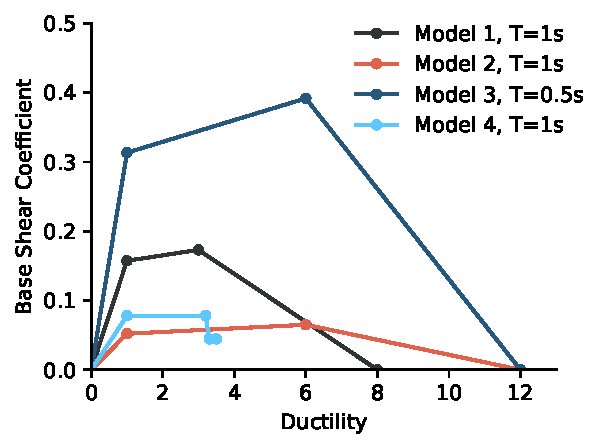
\includegraphics[width=\linewidth]{figs/backbones.pdf}
        \caption{}
        \label{fig:bacbkone}
    \end{subfigure}
    \hfill
    \begin{subfigure}{0.48\textwidth}
        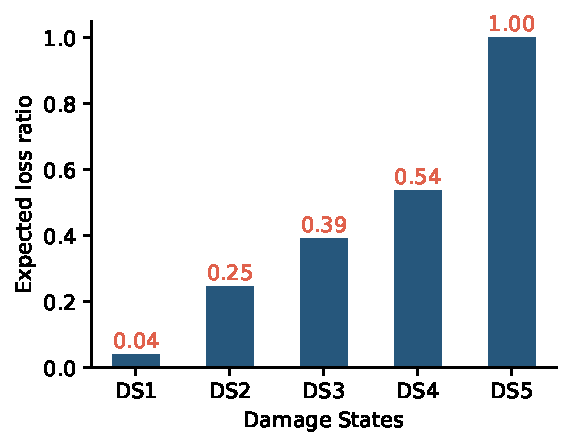
\includegraphics[width=\linewidth]{figs/dmg-model.pdf}
        \caption{}
        \label{fig:damage_model}
    \end{subfigure}
    
    \caption{(a) Backbone curves of the \acp{SDOF} utilised for non-linear dynamic analyses, and (b) damage-to-loss model}
    \label{fig:backbone-damage_model}
\end{figure}


For each structural system, five \acp{DS} were considered. DS1 was assumed to initiate at 75\% of the yielding displacement. Significant damage (DS4) corresponds to the onset of fracturing, while intermediate \acp{DS} were evenly spaced between DS1 and DS4. Complete damage (DS5) was assumed to occur at the system's ultimate displacement capacity. For each of these \acp{DS}, it was assumed that the structure has been damaged to a fraction of its overall replacement value via a \textit{damage-to-loss model}, or \textit{consequence model}. These are denoted $E\left[L\mid DS_i\right]$ for damage state $DS_i$ and when combined with the fragility functions, the expected loss ratio versus intensity is obtained to give the vulnerability function via Equation \eqref{eq:total_loss_gem}. This study adopted the damage-to-loss model from \citet{oreilly-shahnazaryan-2024}, shown in Figure~\ref{fig:damage_model}.

\begin{equation}\label{eq:total_loss_gem}
    E\left[L_T \mid  IM\right] = \sum_i E\left[L\mid DS_i\right]P\left[DS_i\mid IM\right]
\end{equation}


\subsection{Characterisation of seismic hazard}\label{sec:hazard-rs}
To characterise the seismic hazard and select ground motion records for the analysis required to develop the fragility/vulnerability models, \ac{PSHA} was performed using the OpenQuake engine \citep{pagani2014} for the site of L'Aquila, Italy.  In particular, the seismic source model ZS9 proposed by \cite{MelettiEtAl2008} for the seismic hazard assessment of Italy \citep{MStucchi2009,StucchiEtAl2011} was adopted. The adopted ground motion logic tree collapses to a single branch, defined using the \ac{GMM} by \cite{AristeidouEtAl2024_gmm}, developed for active shallow crustal regions. This choice was motivated by the model's ability to predict the next-generation IMs of interest in the present work. The hazard curves for each \ac{IM} previously described are shown in Figure \ref{fig:hz-curves-consistency} and Figure \ref{fig:disaggregation} illustrates a sample disaggregation in terms of both exceedance and occurrence for $Sa(1.0s)$ at 10\% \ac{POE} in 50 years.

\begin{figure}[htbp]
    \centering
    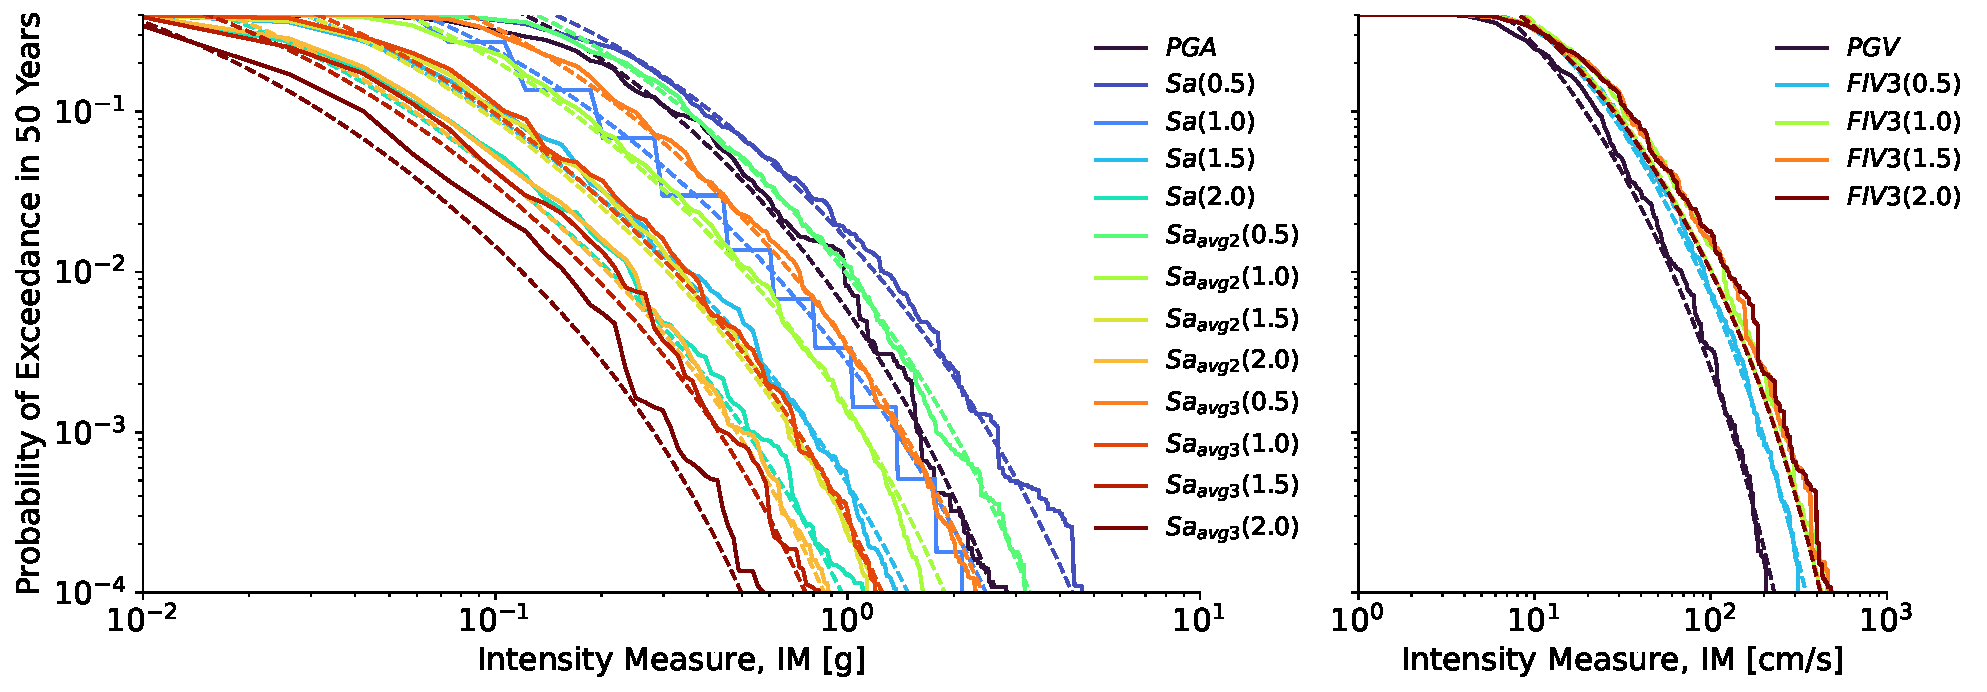
\includegraphics[width=1.0\linewidth]{figs/hzc_SA(1.0).pdf}
    \caption{Hazard curves for each \ac{IM} considered (dashed lines) alongside the hazard consistency checks (solid lines) for the selected ground motion record set conditioned on $IM=Sa(1.0s)$}
    \label{fig:hz-curves-consistency}
\end{figure}


A set of 40 ground motion records (single component) was selected from the NGA West-2 database \citep{Ancheta2014} for each \ac{IM} and \ac{POE} level. These followed the conditional spectrum method using the Djura Record Selector (https://apps.djura.it) \citep{Shahnazaryan2025}. Figure \ref{fig:hz-curves-consistency} also shows the hazard consistency checks for the ground motion record set selected for $IM=Sa(1.0s)$, where a good agreement was observed across all \acp{IM} considered in this study. Similar plots for all other \acp{IM} are available in the GitHub repository.

\begin{figure}[h]
    \centering
    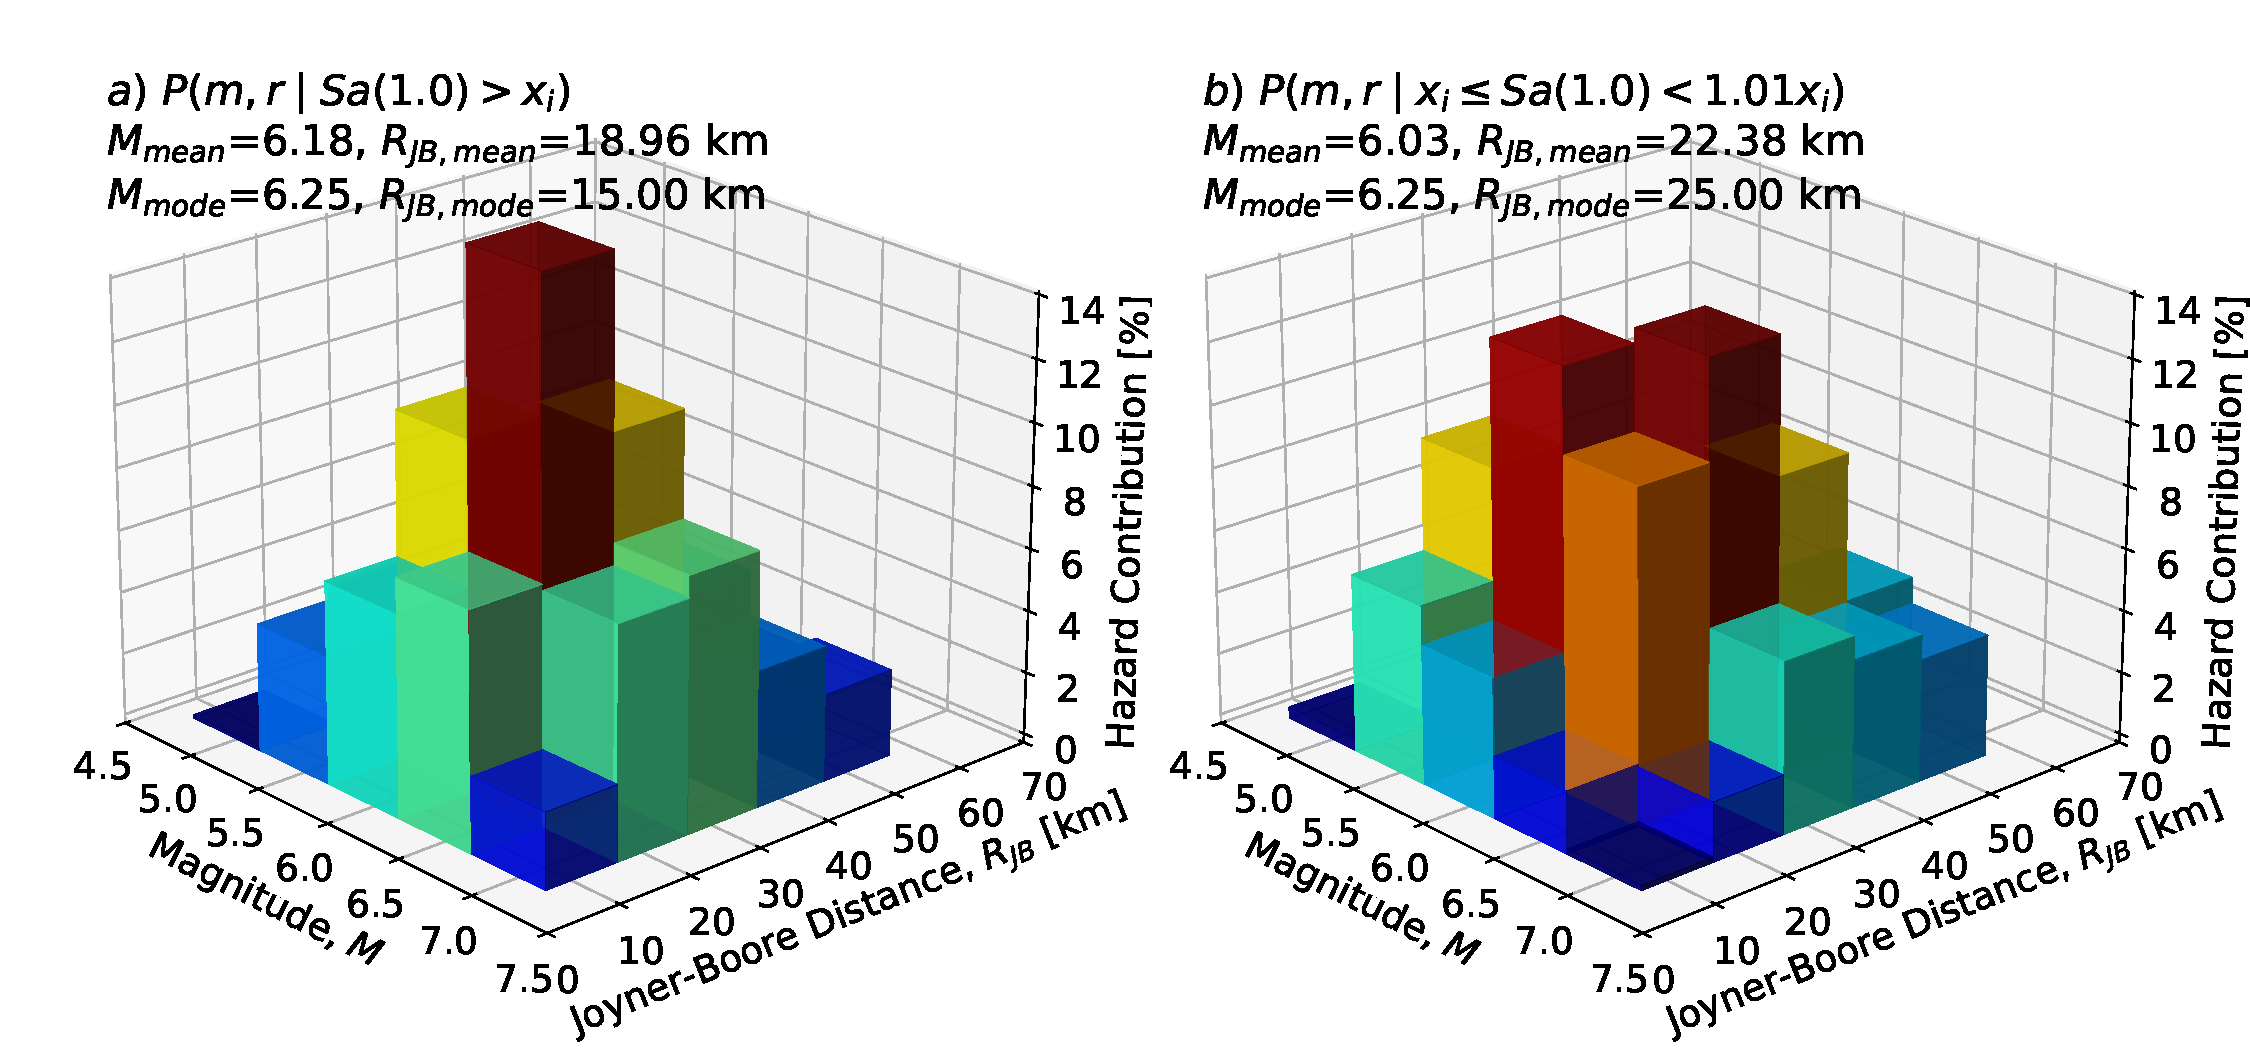
\includegraphics[width=\linewidth]{figs/disagg_SA(1.0)_poe_0.1.pdf}
    \caption{Seismic hazard disaggregation for $Sa(1.0s)$: a) $Sa(1.0s) > x_i$, b) $x_i \leq Sa(1.0s) < 1.01\cdot x_i$ where $x_i = 0.19g$}
    \label{fig:disaggregation}
\end{figure}

\subsection{Numerical analysis and fragility/vulnerability modelling}\label{sec:ff-dev}
\Ac{MSA} was carried out using the ground motion record sets identified in Section \ref{sec:hazard-rs} on the structural systems described in Section \ref{sec:structural-system}. For each structural model, fragility functions were developed for each \ac{DS} considered and ground motion record set. With these \ac{MSA} results for each combination and the \ac{DS} definitions previously described, fragility functions were developed by counting the number of exceedances of system's \ac{DS} threshold at each \ac{IM} level, and fitting a lognormal distribution to the data via maximum likelihood estimation. Likewise, using the damage-to-loss model shown in Figure \ref{fig:damage_model}, the vulnerability functions were also derived using Equation \eqref{eq:total_loss_gem}.


\section{Model conversion results}
\subsection{Fragility function comparisons}
To first examine the comparisons of each method listed in Section \ref{sec:methodology}, Figure \ref{fig:ffs-single-case} shows a single conversion case, where the fragility functions for a single structure's \ac{DS} are converted from $IM_1=Sa(1.0)$ to $IM_2=PGA$ and then compared to the reference fragility function initially developed in terms of $IM_1=PGA$. Also shown for each conversion case are the Hellinger distances, as per Equation \eqref{eq:H-dist}.

In general, there is some variability between the approaches examined, with the most refined approach (Method 1) visually matching closely, as confirmed by the low Hellinger distance. This observation confirms that implementing the total probability approach is indeed effective for converting the \ac{IM} of fragility functions. Methods 2a, 2b, and 2c, which are similar to Method 1 but with much reduced consideration of seismic hazard information, also show good agreement. This confirms the results previously presented in \citet{Suzuki2020}, who performed a similar conversion between these \ac{IM} types, albeit for different structures and seismic hazard. There are some differences but the overall match is quite good. For Methods 3, 4, and 5, on the other hand, their limitations are evident, as the matching is relatively poor for this specific case. This stems from the assumption that the dispersion was equal to the initial $IM_1= Sa(1.0)$ value, despite the fact that a more inefficient $IM_2=PGA$ was being sought; hence, a higher dispersion would have been expected. Methods 1 and 2 captured this shift in dispersion, whereas the other methods did not. Additionally, the median value is quite different, meaning that a simple scaling based on uniform hazard is also not always guaranteed to work and is case specific, as will be shown next. A brief note of caution is made regarding the Hellinger distances shown in Figure \ref{fig:ffs-single-case} since it shows that Methods 2a, 2b, and 2c are apparently more accurate than Method 2 due to the lower value, despite Method 2 being a simpler implementation of Method 1. This difference, while relatively low, was due to the fitting error between the discrete data obtained from each of the conversion methods and the subsequent fitting of a lognormal distribution that was evaluated.

\begin{figure}[htbp]
    \centering
    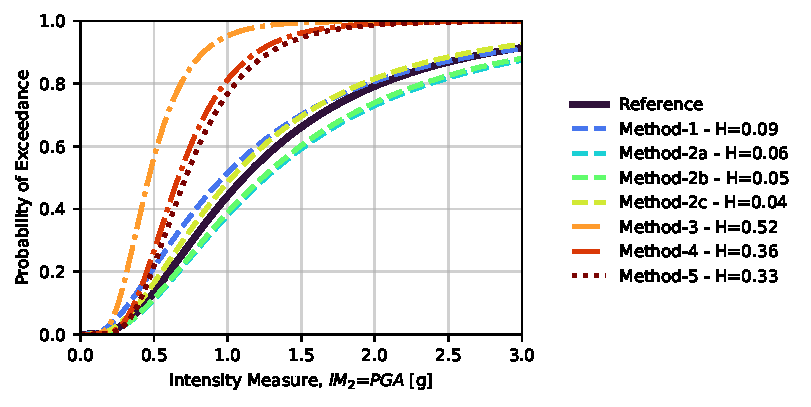
\includegraphics[width=0.8\linewidth]{figs/IM1_SA(1.0)-IM2_PGA-rev.pdf}
    \caption{Comparison of reference ($IM_1=PGA$) and converted (from $IM_1= Sa(1.0)$ to $IM_2=PGA$) fragility functions for Model 2 at DS5}
    \label{fig:ffs-single-case}
\end{figure}

To present a more general view of the methodologies, Figure \ref{fig:ffs-listA} presents a similar conversion using a single model and \ac{DS} but for different $IM_1-IM_2$ pairs. The vertical axis of the plot grid indicates the original $IM_1$ and the horizontal axis indicates the converted $IM_2$, meaning that the first row, second column (starting from the bottom left) shows the case of an $IM_1=Sa(2.0s)$ fragility function converted to $IM_2=Sa(0.5s)$. Overall, the results confirm the observations made in Figure \ref{fig:ffs-single-case}. Methods 3, 4, and 5 tended to match in some cases, particularly when the level of dispersion was similar between the $IM_1-IM_2$ pairs, but worsened as these deviated. This is particularly true for cases where all methods have comparable conversions, making the choice of conversion approach less critical given that next-generation IMs have high efficiency and sufficiency. Methods 1 and 2, on the other hand, showed promising results once again; in particular, the results shown in the lower triangle of the plot grid in Figure \ref{fig:ffs-listA} illustrated very good matching. This corresponds to cases where an $Sa(T)$-based \ac{IM} is converted to a shorter period of vibration (e.g., $IM_1=Sa(1s)$ to $IM_2=Sa(0.5s)$). There is no clear advantage of considering all possible hazard scenarios as required by Method 1, with each variation of Method 2 also illustrating comparable accuracy, indicating that such scrutiny with respect to seismic hazard disaggregation input information may be relaxed when adopting a total probability approach. For the upper triangle of Figure \ref{fig:ffs-listA}, which corresponds to cases where an $Sa(T)$-based \ac{IM} is converted to a higher period of vibration (e.g., $IM_1=Sa(0.5s)$ to $IM_2=Sa(2.0s)$), the accuracy of each conversion methodology tends to break down. This trend was observed for all structures examined at each \ac{DS} considered, where the complete set of plots is available on the GitHub repository. These results also confirm the observations of \citet{Suzuki2020}, who made $Sa(T)$-based conversions from $Sa(T_1)$ to $Sa(T_2)$, and noted that when $T_1 > T_2$ (i.e., the lower triangle case of Figure \ref{fig:ffs-listA}), the results tended to be generally good. When $T_1 < T_2$ (i.e., the upper triangle case of Figure \ref{fig:ffs-listA}), the conversions tended to be quite poor. This was attributed to the fact that, in such cases, the conditional distribution becomes wide and poorly constrained, forcing the conversion integral to operate in extrapolation regions where the scalar IM cannot represent the true structural response. In these cases, Methods 3–5 may at first appear to give more reasonable conversions, but further scrutiny reveals this is an artefact of the constant dispersion assumption, which constrains how poorly these methods can perform and is not a reflection of superior conversion methodology. The result in this case is a false impression of better performance, which in the broader scheme of cases analysed is still rather poor. \citet{Suzuki2020} alleviated this issue by constructing vector-valued fragility surfaces using a hybrid linear–logistic model before performing the conversion, highlighting the need for additional scrutiny when converting to intensity measures at longer vibration periods.

\begin{figure}[htbp]
    \centering
    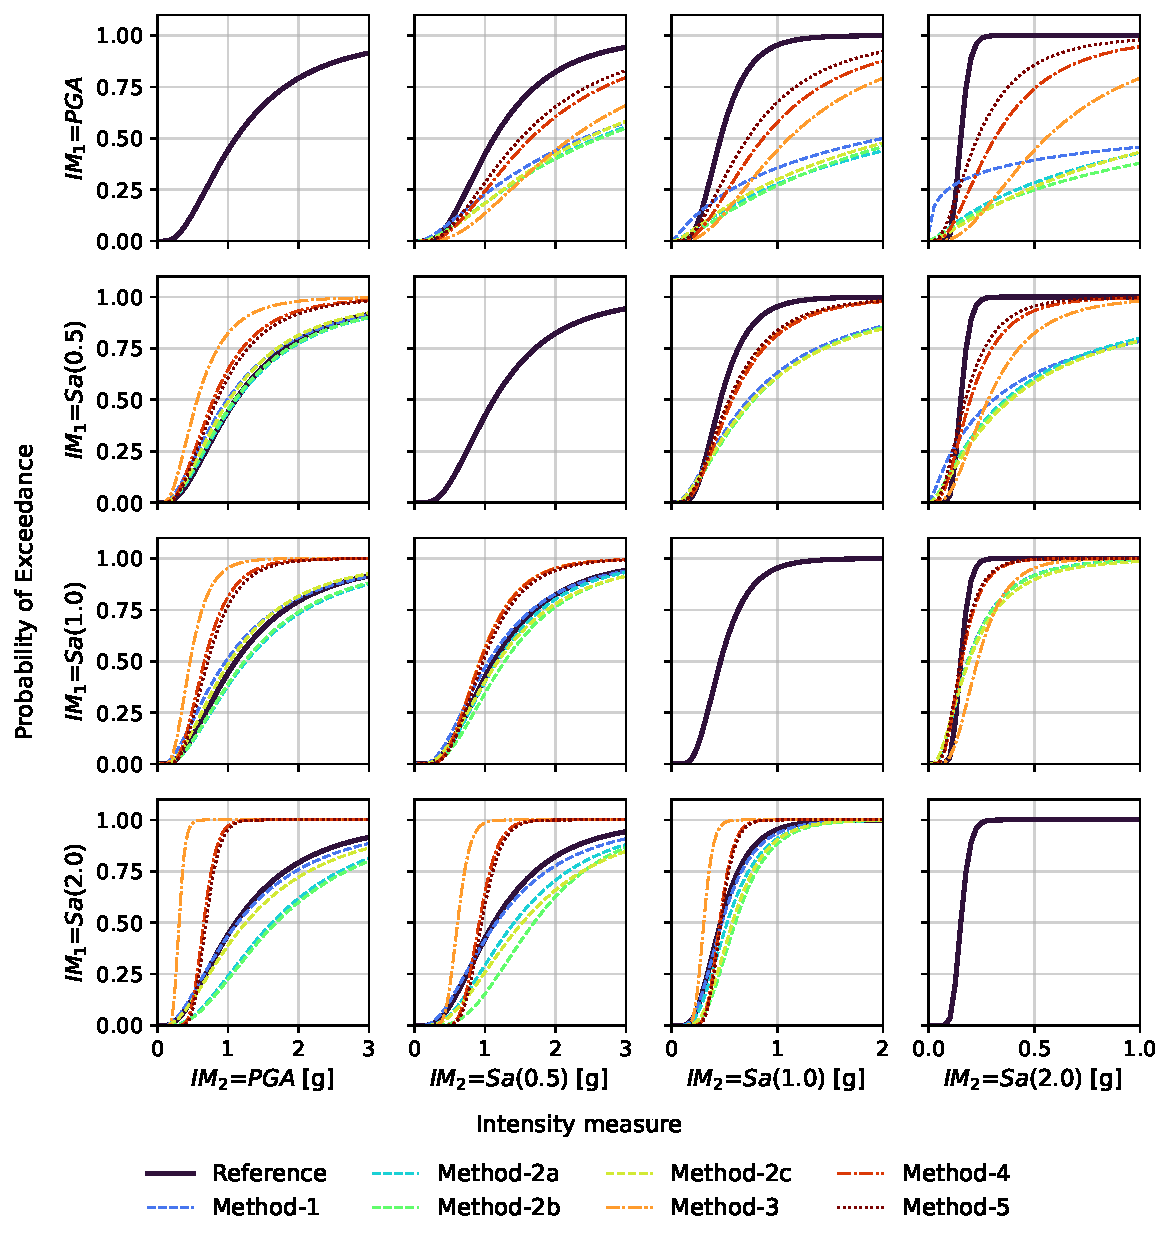
\includegraphics[width=1.0\linewidth]{figs/ff-multi-listA-model_2_ds_5.pdf}
    \caption{Comparison of reference and converted fragility functions for Model 2 at DS5 using traditional \acp{IM} such as $PGA$ and $Sa(T)$}
    \label{fig:ffs-listA}
\end{figure}


In addition to the $Sa(T)$-based conversion of fragility functions presented in Figure \ref{fig:ffs-listA} and past literature, this study also investigated next-generation \acp{IM} such as $FIV3(T)$ and $Sa_{avg}(T)$, alongside $PGV$. Figure \ref{fig:ffs-listB} illustrates some of these conversion cases for a single structure and \ac{DS}, but the overall trends were observed to be similar for the other cases not presented. 

First, examining the methods (excluding Method 3, since it converts only $Sa(T)$-based \acp{IM}), it is clear that each conversion strategy achieves a similar level of accuracy across almost all cases. That is, whereas Methods 4 and 5 tended to perform poorly compared to Methods 1 and 2 when applied to traditional \acp{IM} (Figure \ref{fig:ffs-listA}), Figure \ref{fig:ffs-listB} shows that when converting between next-generation \acp{IM}, there was no significant difference or loss in accuracy. This was found to be due to the much higher efficiency (i.e., lower dispersion) of these next-generation \acp{IM} in characterising the structural damage. Since the overall variability was low across the $IM_1-IM_2$ pairs, simply converting median values under either uniform hazard or risk equivalency was not a bad approximation. Looking at the individual comparisons, $PGV$ is seen to be an \ac{IM} that is relatively easy to convert to, regardless of the method employed. $Sa_{avg2}(1.0s)$ also appeared to be relatively consistent in its conversion results, both to and from. The only case that illustrated sub-par performance was when converting from $IM_1=Sa_{avg2}(0.5s)$ to $IM_2=FIV3(1.0s)$, where the more refined Methods 1 and 2 did not perform so well, especially when compared to Methods 4 and 5, although this is attributed to the same issue of converting from short period \acp{IM} to longer period ones.


\begin{figure}[htbp]
    \centering
    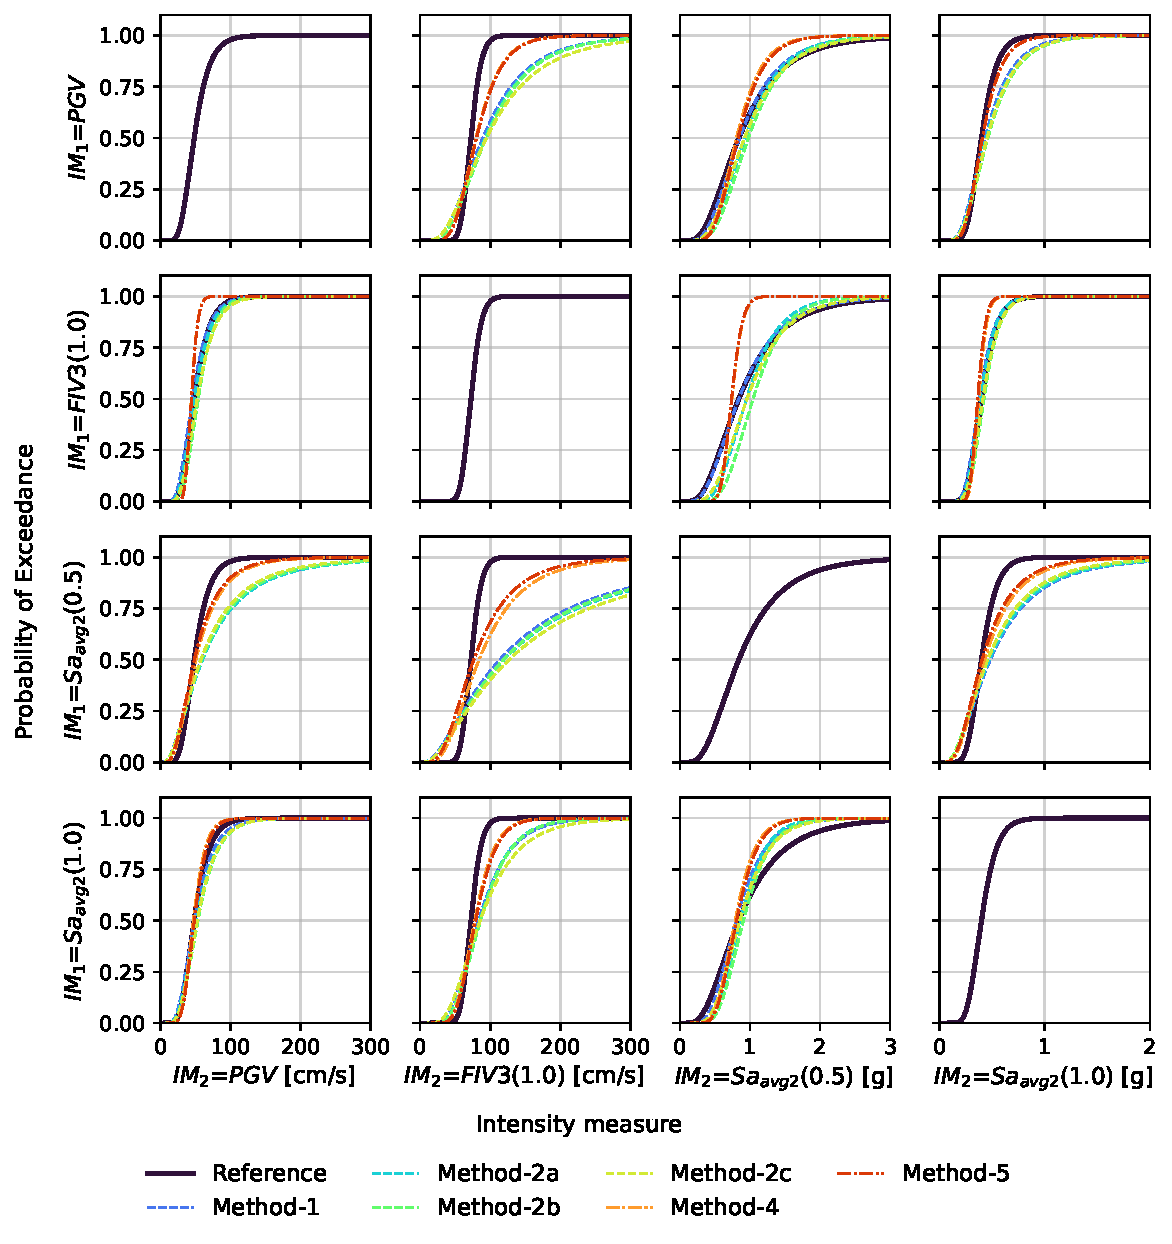
\includegraphics[width=1.0\linewidth]{figs/ff-multi-listB-model_2_ds_5.pdf}
    \caption{Comparison of reference and converted fragility functions for Model 2 at DS5 using next-generation \acp{IM} such as $FIV3$, and $Sa_{avg}(T)$}
    \label{fig:ffs-listB}
\end{figure}


\subsection{Overall results}
% Include this in text: IM2=SA(T1) metrics were excluded in the hellinger distance calculations due to its deterministic nature of damage state CDFs. Only DS5 (collapse) was used. Additionally, for other Period-dependent IMs, the hellinger distances are slightly higher when converting to the IM(T1), this is again in part due to the SDOF system's fundamental period.

While the previous section presented cases of fragility function conversion for specific \ac{IM} pairs within a given structural model and \ac{DS}, this section presents overall comparisons in a more holistic manner using the Hellinger distance described in Equation \eqref{eq:H-dist}. These are plotted in Figure \ref{fig:hellingers} as the average value across each \ac{DS} and method presented, and for all \ac{IM} combinations considered. In short, red indicates a case where the conversion matched poorly to the reference fragility, and green indicates a good conversion. Method 5 is not presented for plotting convenience (although its results are available on the associated GitHub repository), and also since the results closely resembled those of Method 4, which was previously observed in Figures \ref{fig:ffs-listA} and \ref{fig:ffs-listB}.

Overall, when using fragility functions based on $IM_1=PGA$, regardless of the method employed, their conversion to any other $IM_2$ does not work well. This is because of the efficiency and sufficiency issues typically present when using $PGA$, and this loss of information when characterising fragility functions in terms of $PGA$ cannot be recovered when converting to a more effective \ac{IM}. Because of this, it is strongly recommended not to develop fragility models for regional application in terms of $PGA$, as their flexibility is very limited. On the other hand, for most other $IM_1$ types, converting to $IM_2=PGA$ seems to be very feasible, with the exception of Methods 3, 4 and 5. This means that if fragility models are characterised using more efficient \acp{IM} like $Sa(0.5)$ and $Sa(1.5s)$, converting them to a common denominator in $PGA$ is not a bad solution. This is due to the increased explanatory power of these other \acp{IM} that render it suitable to relate to the less accurate $PGA$. The overall variability of the converted fragility functions will still be high, but the conversion methodology should still work well. 

This same observation can also be made for $IM_1=Sa(0.5s)$, where attempting to convert to anything other than $PGA$ is problematic. On the other hand, converting from higher period values of $Sa(T)$ to a lower period tended to work well across the board, where the reverse case was not true, confirming the early comments made in reference to Figure \ref{fig:ffs-listA}. These same comments about intra-\ac{IM} period conversions also apply to $Sa_{avg}(T)$, where converting to lower period values worked well, but to longer periods not. It is worth noting that this applies to cases where $IM_1=IM_2=Sa_{avg}(T)$, since cases where $IM_1=Sa_{avg}(T)$ and $IM_2=Sa(T)$ showed good conversion results, suggesting that the increased efficiency of $Sa_{avg}(T)$ made it a flexible candidate to develop fragility functions initially. 

Conversions between all versions of $FIV3(T)$ are very good, which was somewhat expected given that \citet{Aristeidou2025} has shown it to be an \ac{IM} that is highly correlated with itself for different period values. This means it can almost be considered period-independent, and the results in Figure \ref{fig:hellingers} show that switching between definitions of $FIV3(T)$ was easily done using all methods shown. When scrutinising the conversion between $FIV3(T)$ and other \acp{IM}, a curious observation can be made. It can be seen that when $IM_1=FIV3(T)$, converting to any other $IM_2$ type works very well, regardless of the conversion method adopted, which is completely opposite to the $PGA$ case. To adopt terminology used in blood transfusions, $PGA$ can be thought of as a \textit{universal receiver}, where $FIV3(T)$ can be thought of as a \textit{universal donor}. As before, where it was recommended to avoid developing fragility models in terms of $PGA$, since it offers almost no conversion flexibility and poor efficiency and sufficiency, it is instead recommended to develop fragility models in terms of $FIV3(T)$ since it offers excellent conversion flexibility and has been shown to be an efficient, sufficient and explanatory \ac{IM} in many different contexts \citep[e.g.,][]{Davalos2020, Dvalos2021, Aristeidou2024, Montemayor2025, Montemayor2026}. Its relative period independence means that a single value, such as $T=1s$, could be used for all structural typologies, without much loss in accuracy. 

\begin{figure}[htbp]
    \centering
    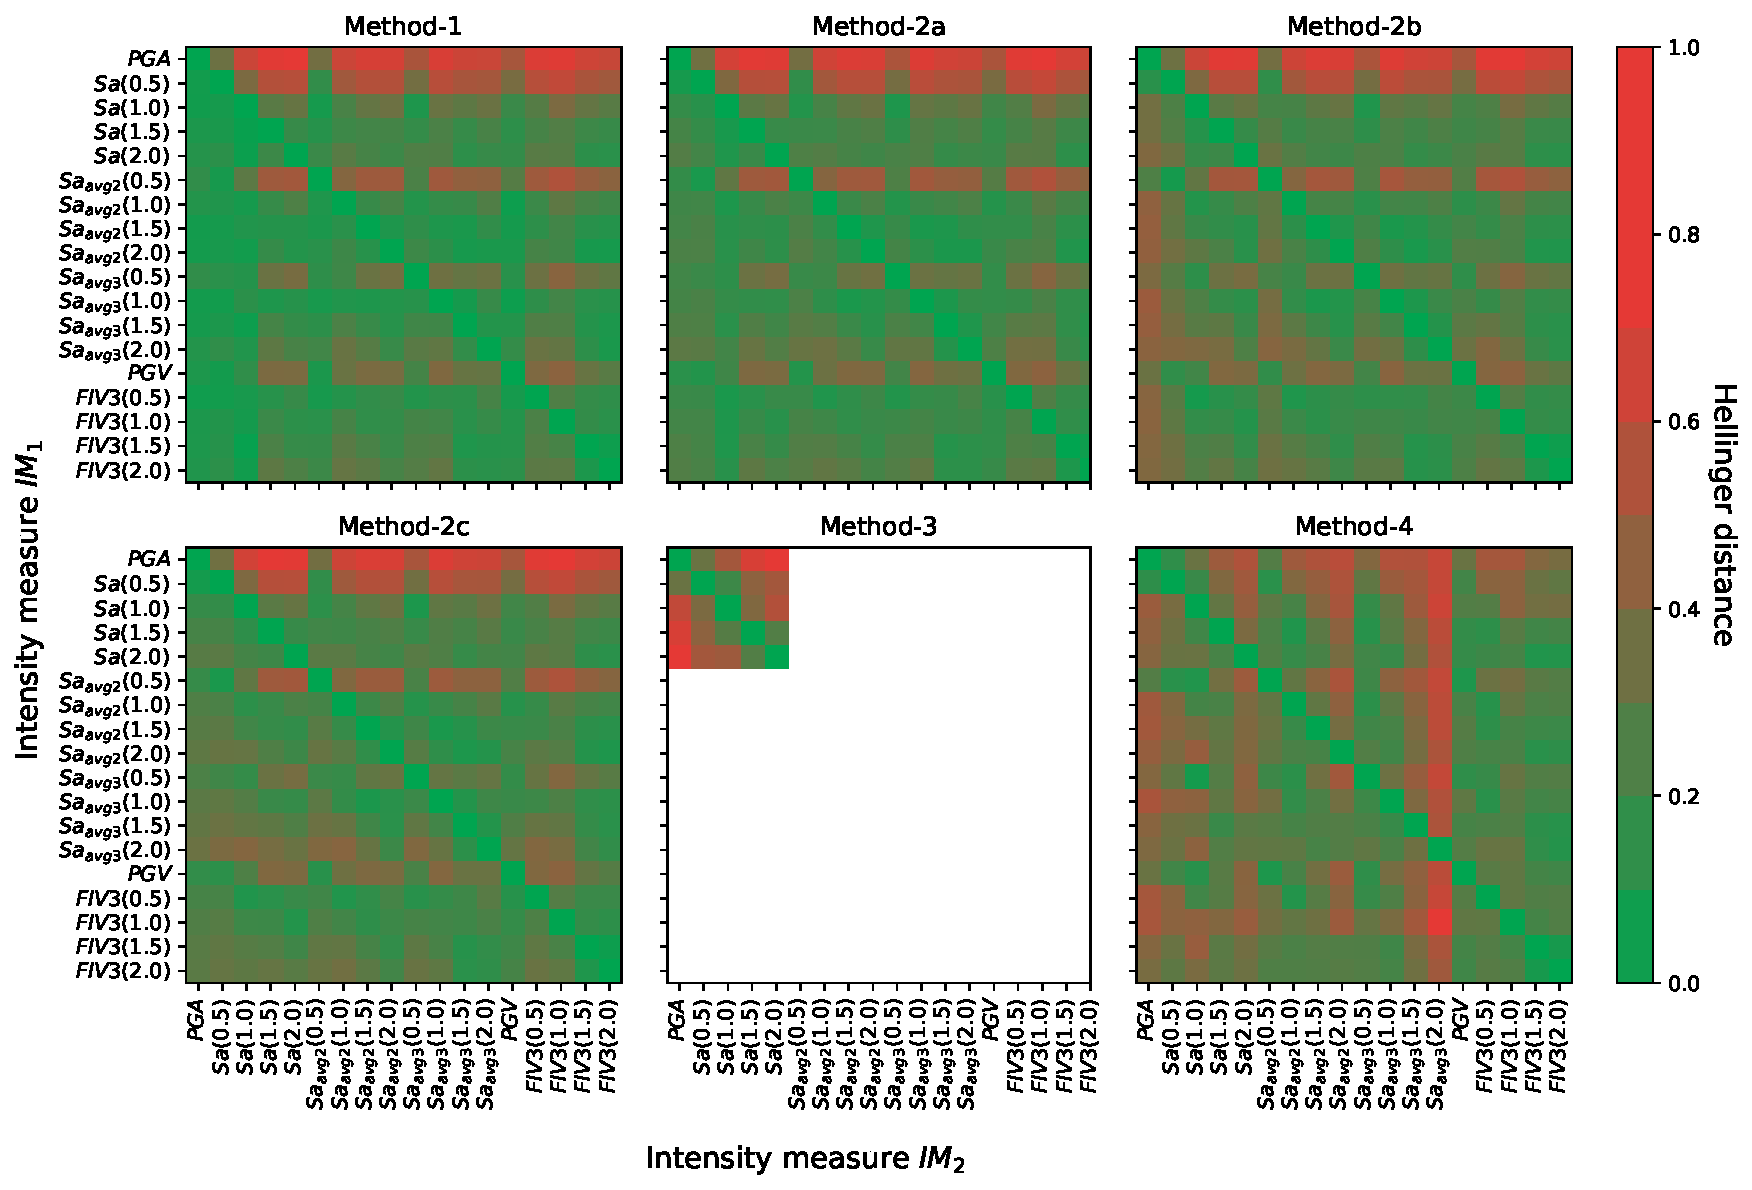
\includegraphics[width=1.0\linewidth]{figs/hellinger-m2.pdf}
    \caption{Average Hellinger distances between the reference and the converted fragility functions (from $IM_1$ to $IM_2$), computed as the mean of distances across DSs, for Model 2}
    \label{fig:hellingers}
\end{figure}

\subsection{Vulnerability functions}
While the previous sections examined the conversion of fragility functions from one \ac{IM} to another, with the different methodologies reviewed in Section \ref{sec:review} exhibiting varying levels of conversion accuracy depending on the case considered, this section extends this consideration to vulnerability functions. This is because, while fragility functions are a key component of seismic risk models, vulnerability models are often presented as the final output when assessing risk and consequences, such as monetary losses. Section \ref{sec:vuln-conversion} described this extension via Equation \eqref{eq:proposed-vf}, where it was illustrated how an original vulnerability function defined as $E[L \mid IM_1]$ can be converted to $E[L \mid IM_2]$ with analogous considerations of hazard and conditional dependence. This was applied using the previously described Methods 1 and 2, and the original vulnerability functions were derived from the original fragility functions using Equation \eqref{eq:total_loss_gem}. 

\begin{figure}[htbp]
    \centering
    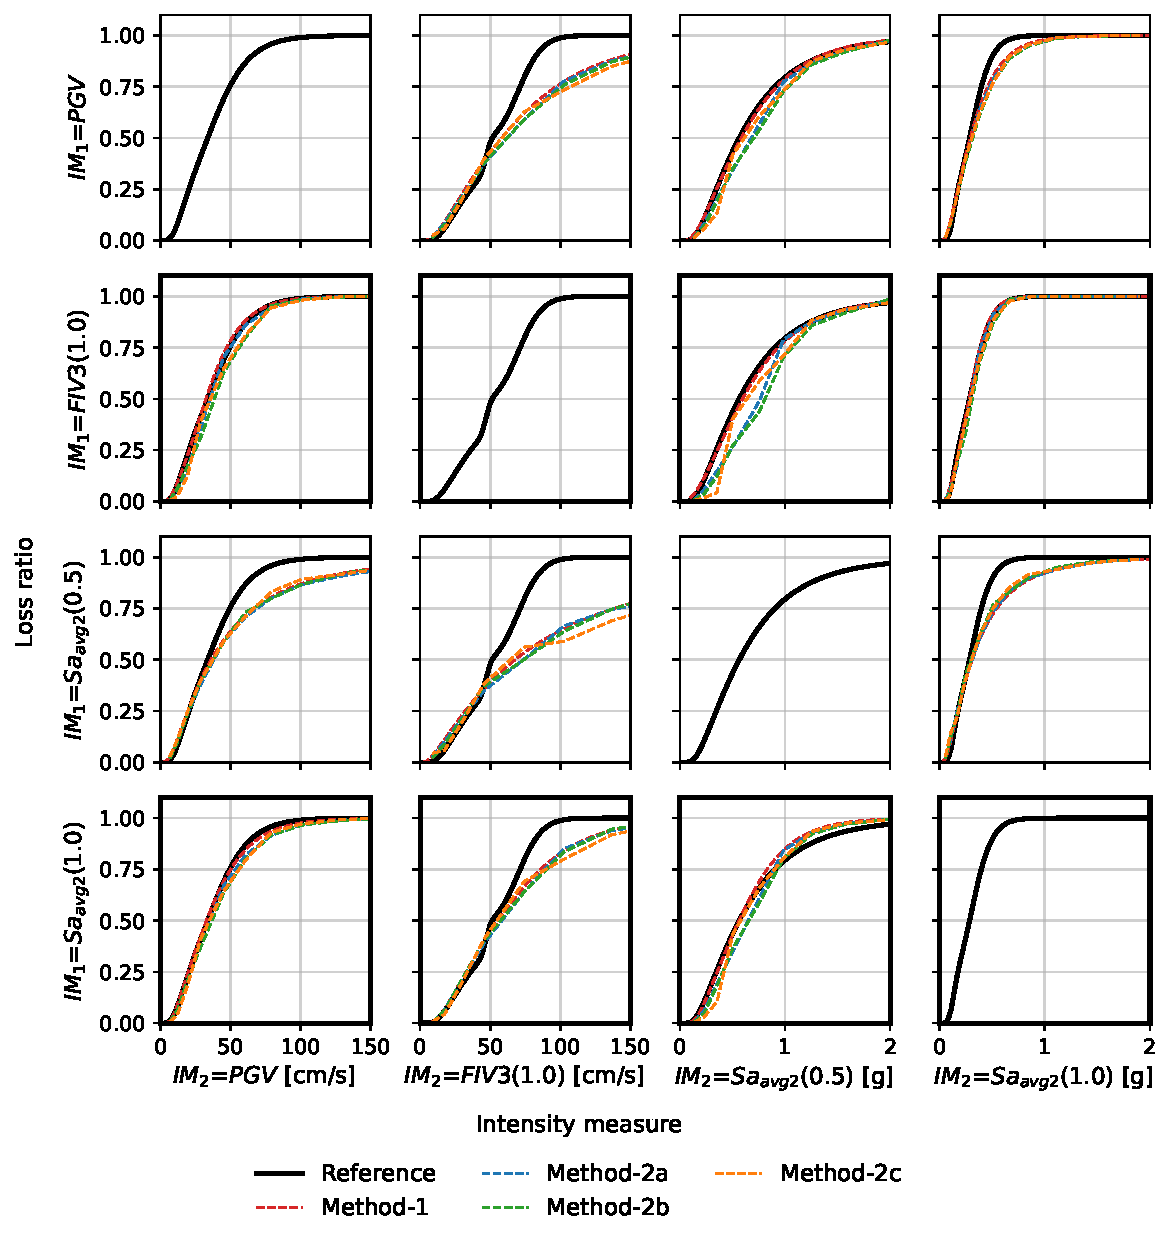
\includegraphics[width=1.0\linewidth]{figs/vf-multi-listB-model_2.pdf}
    \caption{Comparison of reference and converted vulnerability functions for Model 2 using next-generation \acp{IM} such as $FIV3$, and $Sa_{avg}(T)$}
    \label{fig:vfs-listB}
\end{figure}

Figure \ref{fig:vfs-listB} illustrates these comparisons in a way that is analogous to Figure \ref{fig:ffs-listB}. What is immediately apparent is that there is no significant difference between the methods employed, indicating that a simpler consideration of seismic hazard may suffice. Overall, the conversion works quite well when moving between different \acp{IM}. This is much more pronounced in the case of fragility functions, and an encouraging point is that the matching of lower, more frequent intensities seems reasonable in each case. To further understand this, the \ac{AAL} was computed for each case by integrating the vulnerability function with the seismic hazard quantified in Section \ref{sec:hazard-rs}. Figure \ref{fig:delta-aal} shows the difference of the converted vulnerability functions \ac{AAL} with respect to the reference vulnerability function that is being matched. 

Overall, many of the same observations hold, but a notable point again concerns $PGA$. Figure \ref{fig:hellingers} previously showed that converting from $PGA$ to any other \ac{IM} did not work well, but that converting different \acp{IM} to $PGA$ was not a bad solution as they matched the reference model. Figure \ref{fig:delta-aal}, on the other hand, shows that doing this results in a significant overestimation of the \ac{AAL}. This is caused by the increased uncertainty in $PGA$, which increases the expected losses for a given \ac{IM} level, and when integrated with the hazard, inflates the \ac{AAL}. Therefore, the solution of harmonising fragility models in terms of $PGA$ may seem attractive, but when extended to losses and \ac{AAL}, it is shown to grossly overestimate. On the contrary, the previous observation of $FIV3(T)$ being a universal donor \ac{IM} still holds, and maintains good accuracy for the cases examined. Utilising $Sa_{avg}(T)$ as the original \ac{IM} also showed good conversions, further stating the case for these next-generation \acp{IM} to be integrated in vulnerability modelling. All in all, it appears that the vulnerability function conversion is less prone to systematic errors for most \acp{IM} compared to fragility functions, meaning that risk modellers can and may wish to focus their conversion here, rather than fragility, which has been studied to date in the literature.

\begin{figure}[htbp]
    \centering
    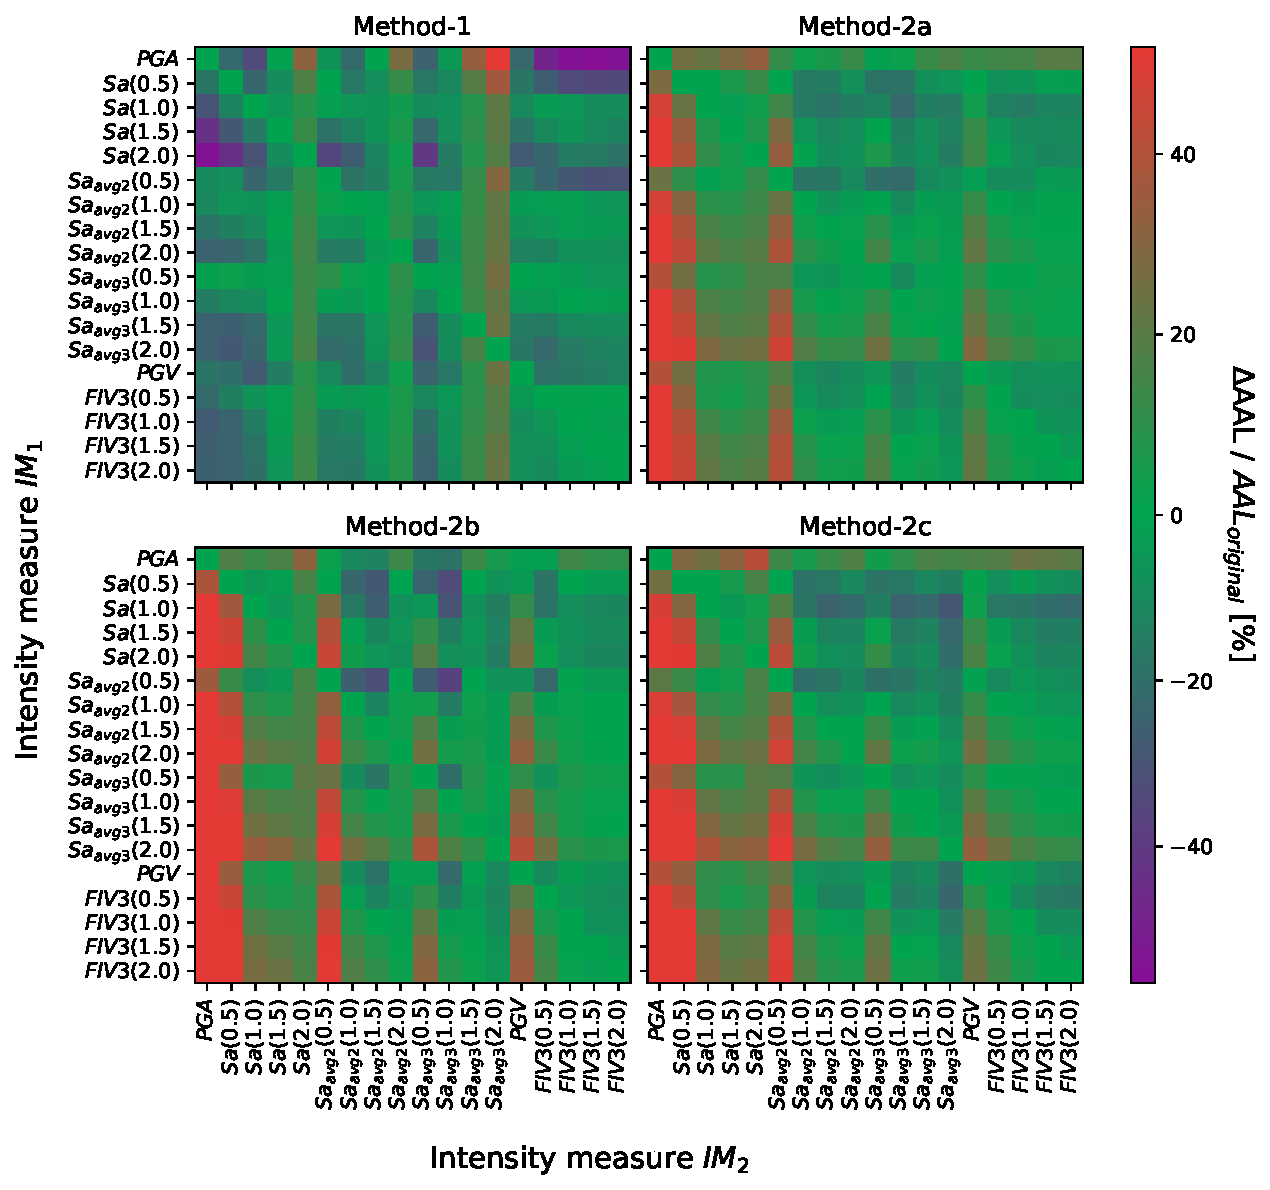
\includegraphics[width=0.9\linewidth]{figs/aal-m2.pdf}
    \caption{\ac{AAL} ratio for vulnerability function conversions $IM_1$ to $IM_2$ for Model 2}
    \label{fig:delta-aal}
\end{figure}

% Some context for the Delta AAL, I chose to show delta AAL instead of delta AAL divided by AAL_original, because the division was a little confusing, as without the actual values, one might think the error is large. The error seems to be in general higher for exact approach (method 1). This is due to having VF converted yielding higher loss values at low IMs. AALs are in general quite low (around 0.1% in average). This is in part due to good systems and relatively low hazard, and low loss model. By increasing AAL, the delta for exact approach lowers, as the VF divergence at low IM values has a lower impact in AAL computation.
% Finally, all methods yielded good results, which is great, meaning one can do a conversion of VF even if detailed disaggregation information is missing.

\section{Remarks}
Overall, there is no single solution to the issues initially outlined. When multiple fragility or vulnerability models are defined using different \acp{IM}, analysts must choose an approach to enable comparison and collective application; in such cases, methods based on total probability should be preferred. Historically, the option of adopting a single \ac{IM} has been common, with $PGA$ being the most widely used over recent decades. However, efficiency and sufficiency considerations have highlighted significant limitations in using $PGA$ to characterise seismic vulnerability. The results presented here further demonstrate how restrictive model definition becomes when using this \ac{IM}, since it complicates fragility function conversion and can substantially overestimate losses when converted models are applied. An alternative is to use next-generation \acp{IM} such as $Sa_{avg}(T)$ or $FIV3(T)$, which retain the practicality of adopting a unique \ac{IM} while avoiding many of the biases and constraints associated with $PGA$. This reinforces the case for future fragility and vulnerability modelling to incorporate these improved \acp{IM}.

The conversion methods investigated employed different strategies, ranging from assumptions of uniform hazard to uniform risk and also the application of total probability. The total probability approach performed best, although it requires more detailed seismic hazard information, which is often available but not always, confirming earlier observations by \citet{Suzuki2020}. Methods 2a, 2b, and 2c, however, indicated that a comprehensive description of hazard disaggregation information is not always needed. Simpler methods can work at times (i.e., Methods 3, 4 and 5), but their success depends heavily on the relative efficiency of the original and target \acp{IM}, which governs the reliability of the conversion. Methods 3 and 4 were expected to perform modestly, which was confirmed. Greater expectations were placed on the feasibility of Method 5, as it is grounded in the principle of uniform risk equivalence; however, this ultimately did not materialise into a usable method. Table \ref{tab:method_comparison} gives an overall summary of each method, noting their required hazard information and other additional models/inputs, their perceived implementation complexity in addition to the relative accuracy observed for the results presented here, provided the initial $IM_1$ is an efficient one. Inevitably, these methods require computational tools for implementation, and some of these tools are provided in the associated GitHub repository, although the challenge of characterising suitable hazard inputs would nevertheless remain to be addressed. 


\begin{table}[ht]
\centering
\caption{Comparison of \ac{IM} conversion methods}
\label{tab:method_comparison}
\footnotesize
\begin{tabular}{|
p{2.0cm}|
p{1.4cm}|
p{1.4cm}|
p{1.4cm}|
p{1.4cm}|
p{1.4cm}|
p{1.4cm}|
p{1.4cm}|}
\hline
 & Method 1 & Method 2a & Method 2b & Method 2c & Method 3 & Method 4 & Method 5 \\
\hline
Required hazard information
& Complete \ac{PSHA} output for $IM_2$
& Complete \ac{PSHA} output for $IM_2$
& Partial \ac{PSHA} output for $IM_2$
& Partial \ac{PSHA} output for $IM_2$
& Uniform hazard spectrum
& Hazard curves for $IM_1$ and $IM_2$
& Hazard curves for $IM_1$ and $IM_2$ \\
\hline
Additional models/inputs
& \acp{GMM} and correlation models
& \acp{GMM} and correlation models
& \acp{GMM} and correlation models
& \acp{GMM} and correlation models
& Dispersion value for $IM_2$
& Dispersion value for $IM_2$
& Dispersion value for $IM_2$ \\
\hline
Implementation complexity
& High
& High
& Moderate
& Moderate
& Low
& Low
& Low \\
\hline
Accuracy
& High
& High
& High
& High
& Moderate
& Moderate
& Low \\
\hline
\end{tabular}
\end{table}


Another important aspect not explored in this study, and which should form the basis of future research, is the issue of site dependence. All fragility or vulnerability functions and conversions here were derived for a single site location. How they extend to other regions with different tectonic environments remains to be confirmed, particularly given the influence of seismic hazard information in the conversion equations. In reality, site dependence also affects current fragility or vulnerability models, although it is seldom discussed. The degree to which these models are independent or sufficient with respect to site hazard depends largely on the chosen \ac{IM}. \citet{Kohrangi2017a} demonstrated site dependence for \acp{IM} such as $Sa(T)$, but also indicated that next-generation candidates like $Sa_{avg}(T)$ may exhibit site independence, offering substantial flexibility. If this finding is confirmed for the present study, the implications would be significant. The first implication is that analysts would be encouraged to adopt more efficient \acp{IM}, which would improve the accuracy of loss estimates. The second implication is that analysts would have greater flexibility when converting between models depending on the application, since earlier results have shown that more efficient \acp{IM} convert more reliably.


\section{Summary and conclusions}
This study examined how seismic fragility and vulnerability functions can be converted between different intensity measures (IMs). It reviewed various approaches available in the literature, ranging from assumptions based on uniform hazard equivalence, to the use of proxy structures, to applications of the total probability theorem. In addition, an alternative method based on the principle of uniform risk equivalence was trialled, along with refinements to the probabilistic approach to incorporate more detailed hazard information and non-spectral IMs such as filtered incremental velocity, $FIV3(T)$ and average spectral acceleration, $Sa_{avg}(T)$. These methods were comparatively discussed and collectively applied to many case study conversion scenarios for evaluation. The results of each possible conversion type were compared against a reference function to assess the efficiency of the conversion methods. This comparison was performed for fragility functions across several damage states, as well as for vulnerability functions describing the economic loss of the structure. Based on this analysis, the following conclusions can be drawn:
\begin{itemize}
    \item Methods based on total probability tended to perform best across all conversions examined and should be employed when possible. Methods based on uniform hazard and uniform risk equivalence tended to be less accurate as they depended heavily on the relative efficiencies of the original IM and target IM. If they were equally efficient, simpler conversions requiring little hazard information worked reasonably well. If the original IM was inefficient, the conversion typically broke down, and not much could be done to convert it to an efficient IM. This was true for traditional IMs like $PGA$ or $Sa(T)$, but next-generation IMs like $Sa_{avg}(T)$ and $FIV3$ showed good robustness when converting between themselves;
    
    \item When using period-dependent IMs, like $Sa(T)$ or $Sa_{avg}(T)$, fragility conversion from a higher period to a lower period tends to work well, but not the other way around, as previously noted by \citet{Suzuki2020};

    \item The previous point implies that converting all spectral-based IMs to $PGA$ is a reasonable solution and serves as a common convergence point for comparative analysis. This was observed to be the case, where accurate conversions to $PGA$ could be made, but this still results in an inefficient IM that, when extended to vulnerability, results in overestimations of economic losses and therefore, is not advised;

    \item A very promising observation was made regarding the use of the next-generation IM $FIV3(T)$, since it has been shown by \citet{Aristeidou2025} to be highly correlated with itself and relatively independent of period, meaning a single definition could be widely applied. The real benefit came from its high efficiency in characterising damage and its sufficiency with respect to site hazard. As the previous point suggests that $PGA$ could be a common convergence point, making it a \textit{universal receiver} to use blood transfusion terminology, $FIV3(T)$ can be thought of as a \textit{universal donor}, since fragility functions developed using this IM can be easily converted to other IMs without any significant implications on accuracy or bias. This restates the case for developing fragility/vulnerability models using such flexible IMs.
\end{itemize}

Lastly, although this work has focused on converting fragility/vulnerability functions to a common \ac{IM} to enable collective analysis using a single ground motion field, recent work by \citet{Monteiro2026b} has introduced several cross‐\ac{IM} spatial correlation models. These models can eliminate the need for such conversions, albeit with a modest increase in computational cost.